\begin{center}
Code at \url{https://github.com/cedrict/fieldstone/tree/master/python_codes/fieldstone_86}
\end{center}

\par\noindent\rule{\textwidth}{0.4pt}

{\sl This stone was developed with input from D. Bont{\'e}}. 
\index{contributors}{D. Bont{\'e}}

\par\noindent\rule{\textwidth}{0.4pt}
%%%%%%%%%%%%%%%%%%%%%%%%%%%%%%%%%%%%%%%%%%%%%%%%%%%%%%%%%%%%%%%%%%%%%%%%%%%%%%%%%%%%%%%%%%%%%%

The rifting of the lithosphere is defined by 2 major steps and relates to 
the sedimentary records in the basins. These two steps are the syn-rift 
and post-rift phases:

\begin{center}
\includegraphics[width=13cm]{python_codes/fieldstone_86/images/synpost}\\
{\captionfont Phases of a rift evolution (from MSc course of M. Seranne, 2013).} 
\end{center}

During the syn-rift phase, the extension is active and thinning down both the 
Crust and Lithospheric Mantle. Also, space is created at the surface during the deformation 
of the top of the crust, allowing sedimentation to occur. During the post-rift phase, 
the extension is no longer active and the evolution is on two fronts: 
(1) the thermal re-equilibration of the Lithospheric Mantle that creates a re-thickening 
of the Lithospheric Mantle and 
(2) a post-rift sedimentation in relation with the isostatic re-equilibration that 
follows the change in thickness of the Lithospheric Mantle.

In 1978, McKenzie presented a quantitative model \cite{mcke78} 
that allows the understanding of the lithospheric evolution related to the creation of a rifting. 
The model of McKenzie considered two steps. The first step (syn-rift) was considered as an 
instantaneous and uniform extension of the lithosphere and crust. The second step (post-rift) 
is the thermal re-equilibration of the thinned down lithospheric mantle, considering that 
(a) the temperature at the end of the pre-rift stage is steady state and (b) the composition 
of the lithospheric mantle and underlying Asthenosphere is equivalent. For the purpose of 
thermal modelling, the initial temperature is defined by a fixed temperature at the surface 
and at the base of the Lithosphere, and the radiogenic heat production is neglected.

\begin{center}
\includegraphics[width=13cm]{python_codes/fieldstone_86/images/eqcurve.jpg}\\
{\captionfont Thermal evolution during rifting. 
Figure by D. Bont{\'e}, after Fig. 1 of McKenzie (1987) \cite{mcke78}.}
\end{center}

Since this early work, the definition of the rifting has been 
refined with the addition of the sediments at the top of the system 
(that have a lower thermal conductivity than the crust), 
the addition of heat production (especially in the upper crust and the sediments), 
and the consideration of a non-uniform extension \cite{roke80}.

The aim of the modelling to be developed here is to observe and characterize the thermal 
evolution (recovery) during the post-rift sequence in two dimension as the lateral heat 
conduction is playing a role in the re-equilibration of the lithospheric Mantle. To obtain 
an even more accurate modelling outcome, two elements have been included in the modelling: 
the heat production and sediment. The heat production is commonly associated with $\sim$40\% 
of the surface heat flow and is mostly located in the upper crust. The sediments, with a lower thermal 
conductivity than the crystalline basement, provide an insulating blanket to the system. 

The evolution and timing of the post-rift  thermal recovery of the Lithospheric Mantle 
is to be considered primarily against the intensity of the perturbation that occurs during 
the syn-rift phase. This perturbation of the lithosphere is commonly described by 
the $\beta$-factor (or stretch factor), which considers the vertical thinning during 
a syn-rifting phase. The $\beta$-factor defines the intensity of the rifting and 
is expressed as the initial thickness divided by the final crustal thickness. 
The higher the $\beta$-factor, the more developed the rifting is with the oceanisation 
occurring for a value of the $\beta$-factor beyond 4.

\begin{center}
\includegraphics[width=13cm]{python_codes/fieldstone_86/images/allenallen}\\
{\captionfont Basins of the rift–drift suite in terms of increasing stretch factor 
and extensional strain rate. \cite{allen2013}.} 
\end{center}

The code solves the diffusion equation in a 2D Cartesian domain. There are 
five materials in the domain: the sediments (\#1), the upper crust (UC, \#2), 
the lower crust (LC, \#3), the mantle lithosphere (ML, \#4) and the asthenosphere (\#5):

\begin{center}
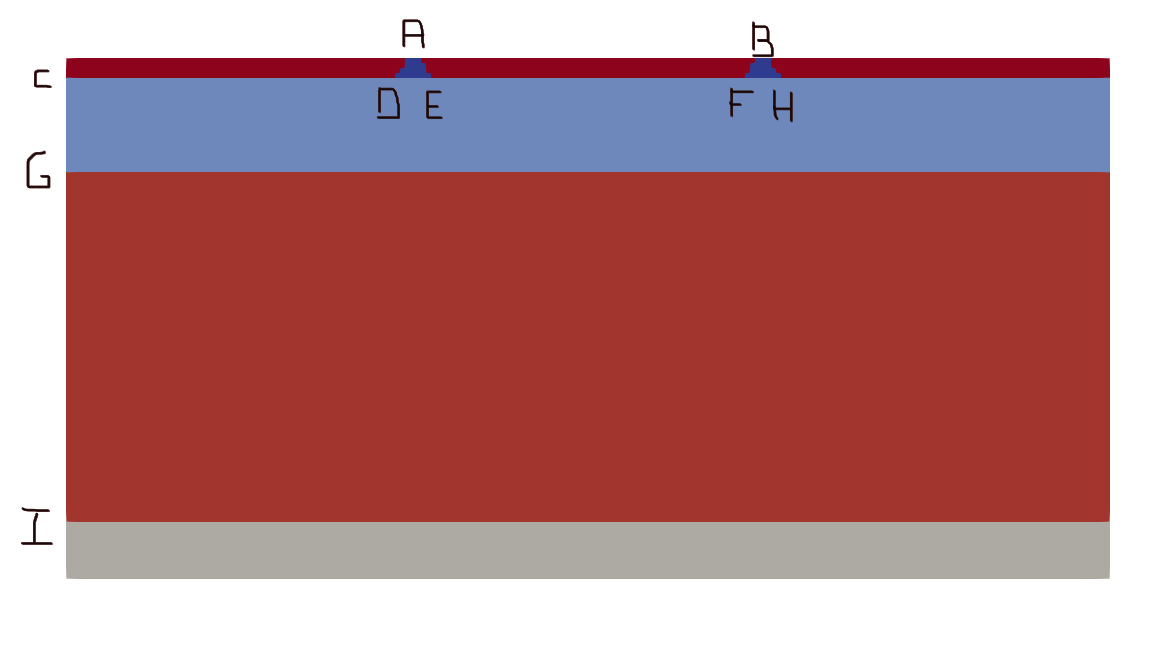
\includegraphics[width=17cm]{python_codes/fieldstone_86/images/setup}\\
{\captionfont Points A..P are used in the code to build the geometry.}
\end{center}

Each material is characterised by its density, its heat capacity, its heat conductivity
and its radiogenic heat production coefficient.

\begin{center}
\begin{tabular}{lllll}
\hline
material & $\rho (\si{\kilogram\per\cubic\metre})$ & $C_p$ & $k$ & $H (10^{-6}\si{\watt\per\cubic\meter})$ \\
\hline
\hline
sediments           & 2100 & 790  & 2   & 0.4-1.8\\ 
upper crust         & 2900 & 1100 & 2.6 & 1.55\\ 
lower crust         & 2900 & 1100 & 2.6 & 0.5\\ 
lithospheric mantle & 3400 & 1260 & 3   & 0\\ 
asthenosphere       & 3400 & 1260 & 3   & 0\\ 
\hline
\end{tabular}
\end{center}


These are the inputs of the code for the geometry:
\begin{itemize}
\item the domain size $L_x$ and $L_y$
\item the thickness of sediments $d_S$
\item the thickness of the upper crust $d_{UC}$
\item the thickness of the lower crust $d_{LC}$
\item the width of the rift $W_R$
\item the width of the taper on each side $w$
\item the three $\beta$ values:
\[
\beta_{UC} =\frac{AM}{BN} =\frac{d_{UC}}{BN}
\qquad
\beta_{LC} =\frac{ME}{NF} =\frac{d_{LC}}{NF}
\qquad 
\beta_{ML} =\frac{EI}{FJ} =\frac{d_{ML}}{FJ}
\]
%\item the coordinates $x_{1..4}$ and $y_{1..6}$
\end{itemize}
Note that the thickness of the lithospheric mantle $d_{LM}$ is simply $d_{LM}=L_y-d_{UC}-d_{LC}$.

This translates as follows in the code:
\begin{lstlisting}
Lx=800e3
Ly=120e3
WR=400e3
w=50e3

d_S=5e3
d_UC=20e3
d_LC=20e3
d_LM=Ly-d_UC-d_LC

beta_UC=2
beta_LC=2.2
beta_LM=2.75
\end{lstlisting}

Concerning the temperature setup, we need to define 5 temperature values:
the temperature at the surface, the temperature at the base of the upper crust,
the temperature at the moho, and the temperature at the LAB.
\begin{lstlisting}
T_surface = 0
T_sediments_base = 200
T_uppercrust_base = 310
T_moho = 550
T_lab = 1330
\end{lstlisting}

%...............................................................................
\paragraph{Steady state} 
If we are only interested in the steady state solution, the equation to solve is then 
simply 
\[
\vec\nabla \cdot k \vec\nabla T + H = 0 
\]
In this case the initial temperature field is irrelevant and so are the heat capacity 
and density values. 
\begin{center}
\includegraphics[width=7cm]{python_codes/fieldstone_86/results/profile_T.pdf}
\includegraphics[width=7cm]{python_codes/fieldstone_86/results/profile_T_top.pdf}\\
\includegraphics[width=7cm]{python_codes/fieldstone_86/results/profile_dTdy.pdf}
\includegraphics[width=7cm]{python_codes/fieldstone_86/results/profile_qy.pdf}\\
{\captionfont top row: Temperature profile at steady state. Bottom row:
vertical temperature gradient and vertical component of the heat flux.} 
\end{center}


\begin{center}
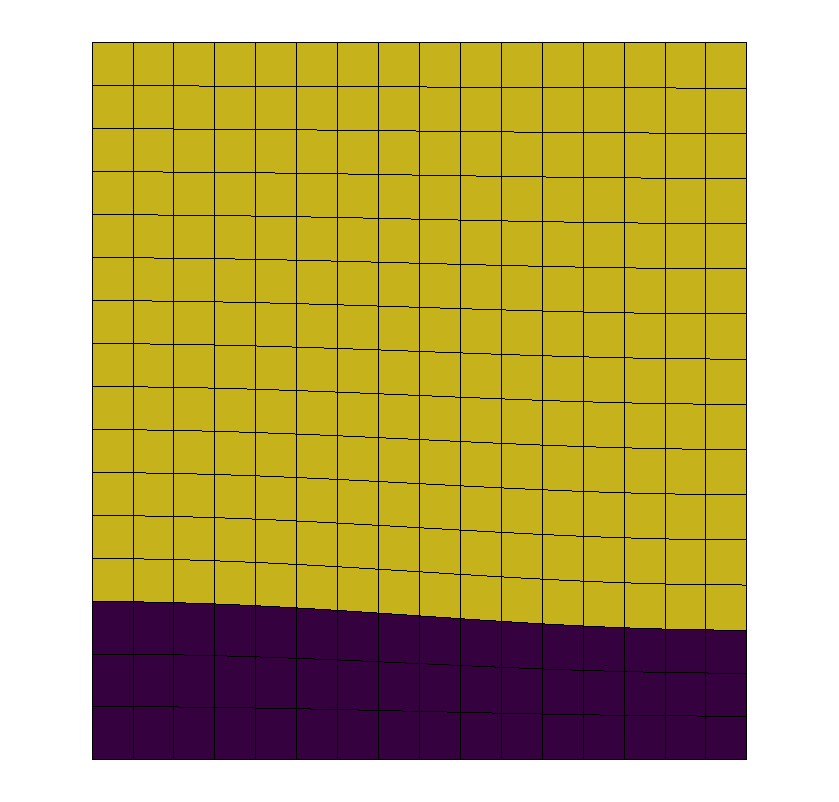
\includegraphics[width=7cm]{python_codes/fieldstone_86/results/mats}
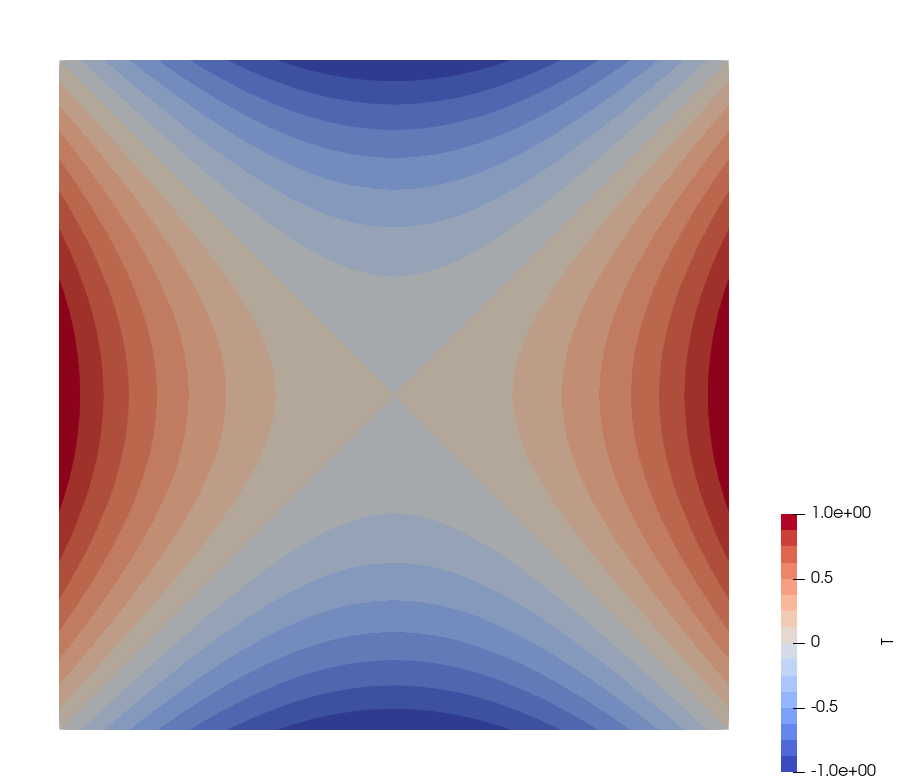
\includegraphics[width=7cm]{python_codes/fieldstone_86/results/T}\\
\includegraphics[width=7cm]{python_codes/fieldstone_86/results/dTdy}
\includegraphics[width=7cm]{python_codes/fieldstone_86/results/heatflux}
\end{center}


ToDo: implement heat source !
